\documentclass[12pt]{book}
\usepackage{hyperref}

\title{Image processing} \author{\url{https://github.com/Grufoony/Physics_Unibo}}
\date{}

\usepackage{amsmath}
\usepackage{amsfonts}
\usepackage{amssymb}
\usepackage{amsthm}
\usepackage{braket}
\usepackage[margin=3cm]{geometry}
\usepackage{pgfplots}
\pgfplotsset{compat=1.18}
\usepackage{fancyhdr}
\usepackage{physics}
\usepackage{systeme,mathtools}
\usepackage{graphicx}
\usepackage{float}
\usepackage{relsize}
\usepackage{calligra}
\usepackage{siunitx}
\usepackage{circuitikz}
\usepackage[miktex]{gnuplottex}
\usepackage{epstopdf}
\usepackage[english]{babel}
\usepackage{float}
\usepackage{tikz}


\newcommand{\vv}{\vec{v}}
\newcommand{\vw}{\vec{w}}
\newcommand{\vo}{\vec{0}}
\newcommand{\vx}{\vec{x}}
\newcommand{\R}{\Re}
\newcommand{\la}{\lambda}
\newcommand{\bd}{\textbf}
\newcommand{\lang}{\left\langle}
\newcommand{\rang}{\right\rangle}
\newcommand{\lbra}{\left\lbrace}
\newcommand{\rbra}{\right\rbrace}
\newcommand{\ih}{\hat{i}}
\newcommand{\jh}{\hat{j}}
\newcommand{\kh}{\hat{k}}
\newcommand{\vr}{\vec{r}}

\begin{document}

\maketitle
\tableofcontents
\pagebreak

\chapter{Introduction to images}
Complex systems are interdisciplinary: you have to communicate your results to experts from different science field.
You need to provide an easy answer to a complex problem, no matter how difficult it's to get this answer.

\section{Emergence}
One of the main ideas in complex systems is emergence. Emergence means that the structure of the particles is simple and they are not so important like interactions bettween them. \\
An example of this is the Central limit theorem, which comes from mathematics. \\ \\
If you have a random variable $x_k$, with average value $\lang x_k \rang = 0$ and finite variance $\sigma^2$, then the central limit theorem says that, if the variables are independent (and in physics this is usally a fair assumption) for every value of $k$, then the normalized sum 
$$
	z_n = \frac{1}{\sqrt{N}}\sum_{k=0}^N x_k
$$
then the distribution of this variable $z_n$ is known, and it is gaussian, for a big enough value of $N$.
$$
	\rho(z_n) \sim \exp\left(-\frac{z^2}{2\sigma^2}\right)
$$
Despite the fact that we, as humans, need a cause-effect relationship to describe a phenomenon, nature loves independent events, like DNA mutations.
The gaussian describes the fluctuations of a system at equilibrium, not the complexity. You cannot extract work from fluctuations at equilibrium, otherwise you violate thermodynamics (and that's no good). \\
The gaussian function is not a physical function, because it implies non zero probabilities to events which are impossible. For example, if we take a particle in a basin of attraction of a potential, the non zero probability given by the gaussian fluctuations allows the particle to jump out of the pit. But this violates the second law of thermodynamics. \\ \\
A way to defy the gaussian properties is to allow a system to have memory, so to remove the independence of the variable. 
\begin{center}
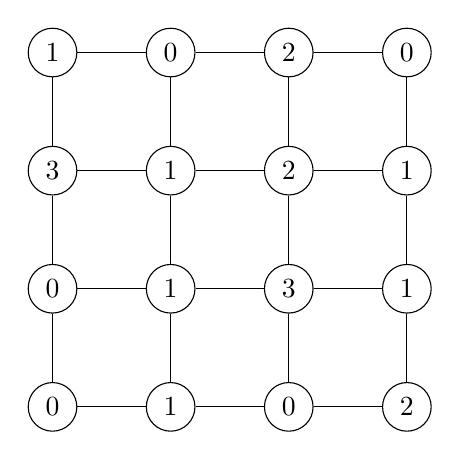
\begin{tikzpicture}[node distance={15mm}, main/.style = {draw,circle}]
\node[main] (1) {1};
\node[main] (2) [right of=1] {0};
\node[main] (3) [right of=2] {2};
\node[main] (4) [right of =3] {0};
\node[main] (5) [below of =1] {3};
\node[main] (6) [right of=5] {1};
\node[main] (7) [right of=6] {2};
\node[main] (8) [right of=7] {1};
\node[main] (9) [below of=5] {0};
\node[main] (10) [right of=9] {1};
\node[main] (11) [right of=10] {3};
\node[main] (12) [right of=11] {1};
\node[main] (13) [below of=9] {0};
\node[main] (14) [right of=13] {1};
\node[main] (15) [right of=14] {0};
\node[main] (16) [right of=15] {2};
\draw (1) -- (2);
\draw (1) -- (5);
\draw (2) -- (3);
\draw (3) -- (4);
\draw (5) -- (6);
\draw (6) -- (7);
\draw (7) -- (8);
\draw (5) -- (9);
\draw (9) -- (10);
\draw (10) -- (11);
\draw (11) -- (12);
\draw (9) -- (13);
\draw (13) -- (14);
\draw (14) -- (15);
\draw (15) -- (16);
\draw (2) -- (6);
\draw (3) -- (7);
\draw (4) -- (8);
\draw (6) -- (10);
\draw (7) -- (11);
\draw (8) -- (12);
\draw (10) -- (14);
\draw (11) -- (15);
\draw (12) -- (16);
\end{tikzpicture}
\end{center}
One example of this is the sand pile model. You have a lattice, and each point is connected to its four neighbors. At this point one particle is put in a randomly chosen point. Each node can have four possible states, $0,1,2,3$, that is four possible numbers of particles. If a node reaches 4 particles, the 4 particles are distributed to the 4 neightbouring nodes.
\begin{center}
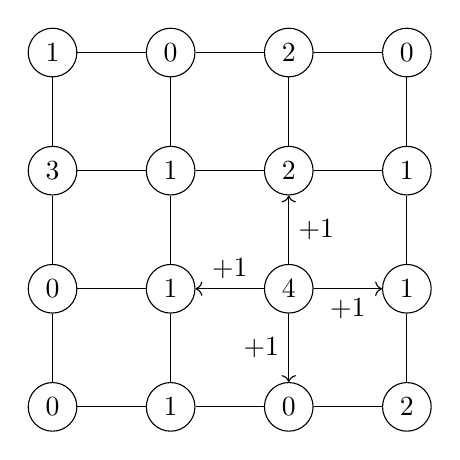
\begin{tikzpicture}[node distance={15mm}, main/.style = {draw,circle}]
\node[main] (1) {1};
\node[main] (2) [right of=1] {0};
\node[main] (3) [right of=2] {2};
\node[main] (4) [right of =3] {0};
\node[main] (5) [below of =1] {3};
\node[main] (6) [right of=5] {1};
\node[main] (7) [right of=6] {2};
\node[main] (8) [right of=7] {1};
\node[main] (9) [below of=5] {0};
\node[main] (10) [right of=9] {1};
\node[main] (11) [right of=10] {4};
\node[main] (12) [right of=11] {1};
\node[main] (13) [below of=9] {0};
\node[main] (14) [right of=13] {1};
\node[main] (15) [right of=14] {0};
\node[main] (16) [right of=15] {2};
\draw (1) -- (2);
\draw (1) -- (5);
\draw (2) -- (3);
\draw (3) -- (4);
\draw (5) -- (6);
\draw (6) -- (7);
\draw (7) -- (8);
\draw (5) -- (9);
\draw (9) -- (10);
\draw[->] (11) -- node[above]{+1} (10);
\draw[->] (11) -- node[below]{+1} (12);
\draw (9) -- (13);
\draw (13) -- (14);
\draw (14) -- (15);
\draw (15) -- (16);
\draw (2) -- (6);
\draw (3) -- (7);
\draw (4) -- (8);
\draw (6) -- (10);
\draw[->] (11) -- node[right]{+1} (7);
\draw (8) -- (12);
\draw (10) -- (14);
\draw[->] (11) -- node[left]{+1} (15);
\draw (12) -- (16);
\end{tikzpicture}
\end{center}
\begin{center}
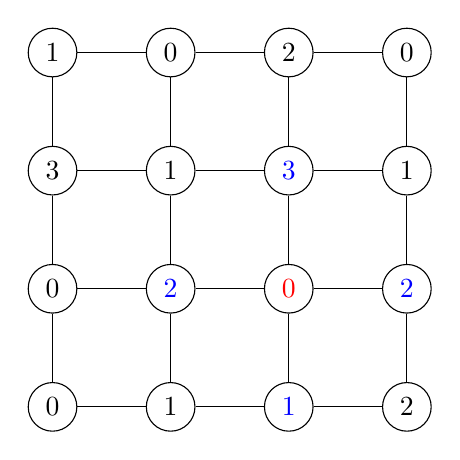
\begin{tikzpicture}[node distance={15mm}, main/.style = {draw,circle}]
\node[main] (1) {1};
\node[main] (2) [right of=1] {0};
\node[main] (3) [right of=2] {2};
\node[main] (4) [right of =3] {0};
\node[main] (5) [below of =1] {3};
\node[main] (6) [right of=5] {1};
\node[main] (7) [right of=6] {\textcolor{blue}{3}};
\node[main] (8) [right of=7] {1};
\node[main] (9) [below of=5] {0};
\node[main] (10) [right of=9] {\textcolor{blue}{2}};
\node[main] (11) [right of=10] {\textcolor{red}{0}};
\node[main] (12) [right of=11] {\textcolor{blue}{2}};
\node[main] (13) [below of=9] {0};
\node[main] (14) [right of=13] {1};
\node[main] (15) [right of=14] {\textcolor{blue}{1}};
\node[main] (16) [right of=15] {2};
\draw (1) -- (2);
\draw (1) -- (5);
\draw (2) -- (3);
\draw (3) -- (4);
\draw (5) -- (6);
\draw (6) -- (7);
\draw (7) -- (8);
\draw (5) -- (9);
\draw (9) -- (10);
\draw (11) -- (10);
\draw (11) -- (12);
\draw (9) -- (13);
\draw (13) -- (14);
\draw (14) -- (15);
\draw (15) -- (16);
\draw (2) -- (6);
\draw (3) -- (7);
\draw (4) -- (8);
\draw (6) -- (10);
\draw (11) -- (7);
\draw (8) -- (12);
\draw (10) -- (14);
\draw (11) --  (15);
\draw (12) -- (16);
\end{tikzpicture}
\end{center}
For the nodes in the border, what happens is that 2 of the particles are redistributed and the other 2 are released in the enviroment, so they are lost. \\ \\
So this system has memory, and this means that the states of all the nodes are not independent. This memory turns the gaussian distribution into a power law
$$
	p(n) \propto n^{-\alpha}
$$
with $\alpha > 1$. \\
The decay of the power low is much slower than that of the gaussian, which means that the probability to have events in the extremes is significantly higher with the power low distribution.
Memory is related to power laws, but vice versa is not guaranteed.
We can also have power laws in physics, for example in the Ising model.
In physics, power laws typically represent a phase transition for a dynamic system in a non-equilibrium state. \\
In the sand pile model, we notice a self-organized criticality: the system naturally goes into a critical state and does a phase transition. \\
Another example of a natural power law is the Kleiber law which relates the metabolic rate (amount of energy you need to survive) to the mass.
\begin{equation}
	E(m) \propto m^{\frac{4}{3}}
\end{equation}
We can also observe that heartbeat rate decreases with mass and lifetime increases.
\section{The broken stick model}
Let's consider the portion $[0,1]$ of the axis, which represents a segment (a stick) of length 1. Suppose that we extract randomically a point $x_1$ on that segment, and we cut it in correspondence of that point, thus obtaining the portion $[0,x_1]$ of the axis. \\
By repeating this process many times, we obtain a system with memory, because of course the length of the segment at a certain iteration depends on all the previous iterations. \\
This is called the broken stick model. \\
For this system one expects to have a power law distribution, because if we rescale the variable $x$, the distribution must not change.
$$
	p(x) \sim \frac{1}{x^a}
$$
$$
	y = \la x \ \ \longrightarrow \ \ p(y) = \frac{1}{(\la x)^a} \sim \frac{1}{x^a}
$$
Since we have:
$$
	\lang x_k \rang = \frac{\lang x_{k-1} \rang}{2}
$$
$$
	\rho_N(2x) = \frac{1}{2}\rho_{N-1}(x)
$$
Which means that, as $N$ goes to infinity we get
$$
	\rho(2x) = \frac{1}{2}\rho(x)
$$
$$
	\rho(x) = \frac{1}{x}
$$
Let's now try to implement the system without memory. So we have $N$ independent variables $x_k$ uniformly distributed, and for each variable we define its distance from the previous one, $\Delta x$. \\
The probability to find $\Delta x$ is the probability of not finding $x$ in any segment, so
$$
	p(\Delta x) \approx \left( 1 - \frac{\Delta x}{L} \right)
$$
We then take a new variable $y = N\Delta x$ and we obtain the probability distribution
$$
	p = \exp(-y/L)
$$
as $N$ goes to infinity, which of course is an exponential law. \\ \\
Suppose that the whole stick is a state, and we want to distribute the population inside of it. If we divide the stick uniformly in portions and diivde the populations in this group, we obtain an exponential law, as we have just seen. \\
Another way, which contains memory, consists of creating a city and letting it grow, and only then introducing a second one, and repeating the process until all the space is occupied. 
\chapter{Total energy in a network}
Let's take a region of space containing a number $N$ of nodes. This system can represent, for example, the hydraulic network of a city. 
For a node we define its ``energy'' flow $\varphi$ (in the case of the hydraulic network, what is flowing between the nodes is water). How much ``energy'' do we need to insert in the system? \\
If we have to distribute something to all the nodes, the most basic way to do it is to connect one on one all the nodes, as to form a long chain. \\
\begin{center}
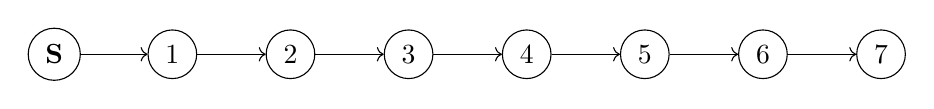
\begin{tikzpicture}[node distance={15mm}, main/.style = {draw,circle}]
\node[main] (1) {1};
\node[main] (0) [left of=1] {\textbf{S}};
\node[main] (2) [right of=1] {2};
\node[main] (3) [right of=2] {3};
\node[main] (4) [right of =3] {4};
\node[main] (5) [right of =4] {5};
\node[main] (6) [right of=5] {6};
\node[main] (7) [right of=6] {7};
\draw[->] (0) -- (1);
\draw[->] (1) -- (2);
\draw[->] (2) -- (3);
\draw[->] (3) -- (4);
\draw[->] (4) -- (5);
\draw[->] (5) -- (6);
\draw[->] (6) -- (7);
\end{tikzpicture}
\end{center}
If the flow out of the source $S$ is $\phi$, the flow after the first node is $\phi - \varphi$, and so on, and we expect that the flow arriving to the final node will be $\varphi$. \\
So the total energy is 
$$
	E_T \approx l\sum_{k=0}^{N-1} (\phi - k\varphi) = l\varphi\sum_{k=0}^{N-1} k`
$$
$$
	E_T \propto l\varphi N^2
$$
So the totaly energy that is required to provide for all the nodes, with this configuration, is proportional to the square of the total number of nodes. So with this configuration we have a network that is very easy to implement, but the network is very inefficient. \\ \\ 
Another possible connection of the nodes is the following one:
\begin{center}
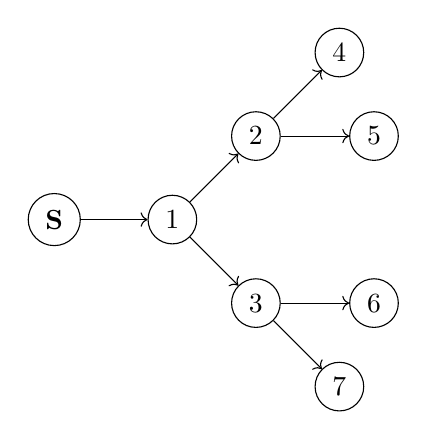
\begin{tikzpicture}[node distance={15mm}, main/.style = {draw,circle}]
\node[main] (1) {1};
\node[main] (0) [left of=1] {\textbf{S}};
\node[main] (2) [above right of=1] {2};
\node[main] (3) [below right of=1] {3};
\node[main] (4) [above right of =2] {4};
\node[main] (5) [right of =2] {5};
\node[main] (6) [right of=3] {6};
\node[main] (7) [below right of=3] {7};
\draw[->] (0) -- (1);
\draw[->] (1) -- (2);
\draw[->]  (1) -- (3);
\draw[->]  (2) -- (4);
\draw[->]  (2) -- (5);
\draw[->]  (3) -- (6);
\draw[->]  (3) -- (7);
\end{tikzpicture}
\end{center}
So each node is linked to two mode nodes. This is what is called a tree structure. \\
The main problem with such a structure is that the path between the nodes is always the same, but it is impossible to design a city in such a way. \\
The number of nodes is $N = 2^{m+1}$, where $m$ is the number of levels. \\
The relation for the flow in each level is
$$
	2\phi_k + \varphi = \phi_{k-1}
$$
where we assume again that the flow in the final level is $\varphi$. \\
$\phi_k$ then is
$$
	\phi_k = (2^{m+1-k}-1)\varphi
$$
Then:
$$
	E_T = d\varphi\sum_{k=1}^m 2^k(2^{m+1-k}-1) \approx d\varphi m 2^{m+1}	
$$
$$
	E_T = d\varphi N \log_2N
$$
This configuration is much more efficient than the previous alternative, although it is impossible to put to practice. \\ \\ 
So we need to find a solution that is in the middle of these two. \\ \\
Another possible structure consists of connecting all the nodes to the source, making a star network: also this model is of course impossible to put in practice. \\
However, in this case the total energy required is proportional to $NL$, where $L$ is the scale length of the system. 
$$
	E_T \propto NL
$$
The proportionality to $L$ is due to the fact that the average length of the links is proportional to the size of the space. \\
Since 
$$
	N = \left(\frac{L}{l} \right)^D
$$
where $D$ is the system dimension (e.g. 1D, 2D...).
We have that
$$
	E_T \propto N\overline{L} \approx N^{1+1/D} = V^{\frac{D+1}{D}}
$$
We notice that:
\begin{itemize}
	\item for a 2D system, like a city, $E \propto V^{\frac{3}{2}}$
	\item for a 3D system, like biological systems, $E \propto V^{\frac{4}{3}}$
\end{itemize}
In any case the exponent is greater than one so, soon or later, the system will collapse.
The problem is also logistic, because in a real transportation line there is also waste, that has to be disposed of. \\ \\
If we consider our system to be an animal's body, this would mean that in order to survive the amount of blood in its body must grow with the size by an amount of $4/3$. This would mean that very big animals can't survive, but they do, and the solution is in Kleiber's law. \\
As animals get bigger, their demand of energy goes down, so their metabolism slows down.  



Once we have a model (which hopefully is a good one), the model is deterministic, so if we know the initial conditions os the system, we know exactly what state the system will have at any future time. \\
The problem with this is that we don't know the initial conditions with absolute certainty. So at this point the question, that will be answered later, is: \\
How much error in the initial conditions is acceptable before that the previsions of our model start to diverge from the real evolution in an unacceptable way?
	













\chapter{Digital images}
When talking about digital images, we must define the concepts of geometry and radiometry. \\
Geometry is the relationship between location and size of the objects in the 3D world and their representation in the image plane. \\
Radiometry is the relationship between the amount of light radiating from a point and the amount of light impinging on the correspondend image point. \\ \\
The most basic image formation device (and the first one historically) is the pin-hole camera. The pin-hole camera consists of a closed room with a small hole (of the order of the millimiter) in one of the walls. When the light coming from the object reaches the hole, the image is formed upside down in the opposite wall of the chamber. The size of the image in the image plane depends on the object's distance from the pin-hole. \\ \\ 
If a point $M$ in the 3D space is characterized by 3 coordinates $(x,y,z)$, the image point in the image plane is characterized by 2 coordinates $(u,v)$. The two sets of coordinates are related by the geometrical equations
$$
	u = \frac{fx}{z} \ \ \ \ \ \frac{fy}{z}
$$
All the light rays are considered to be parallel to the optical axis and orthogonal to the image plane. \\
We define $\Delta z$ as the size of the object with respect to its distance from the camera, so as its thickness. Then, if $2\Delta z$ is small with respect to $z_0$, we have that
$$
	\frac{f}{z_0 + \Delta z} \approx \frac{f}{z_0-\Delta z} \approx \frac{f}{z_0}
$$
which means that
$$
	u\approx \frac{f}{z_0}x \ \ \ \ \ v \approx \frac{f}{z_0}y
$$
This approximation of course is only valid for small objects, or objects that are close to the optical axis. \\
The quality of the image depends heavily on the size of the hole. 
\begin{itemize}
	\item If the hole is too big, we have that a point of the object becomes a spot in the image. This means that the image is going to be blurry. 
	\item If the hole is too small, we can have diffraction effects, that again, end up blurring the image.
\end{itemize}
The solution for balancing the effects of big and small pinholes and settling for a middle ground is in the use of lenses. \\ \\
Lenses have two main strengths: They allow to gather light coming from a point on the object and focus it into a single point on the image; since the aperture size of the lense is larger than that of a pinhole, the exposure times can be reduced as well. \\
Lenses solve another problem as well: In a pinhole camera, we have that many points from the object space are mapped into a single in the image plane. So, an image on the image plane can come from several objects in the real space. \\
On the other hand, a lens brings into focus only those object points that lie within one particular plane parallel to the image plane. \\
So, when the distance between lens and image plane is equal to $v$, only those points that are at a distance $u$ are brought into focus, with $u$ give by
$$
	\frac{1}{u} + \frac{1}{v} = \frac{1}{f} -> u = \frac{vf}{v-f}
$$
In other words, if we bring an object into focus at a distance $u$, we must set the distance $v$ between the image plane and the lens to
$$
	v = \frac{uf}{u-f}
$$
The object points that do not lie within this plane end up being blurred. \\ \\
In a real camera ther is an object called diaphragm, whose purpose is to control the opening of the lens. By reducing the size of the aperture, it reduces the amount of light that reaches the sensor, and also reduces the size of the circle of confusion, thus increasing the depth of field. \\
The \textit{field of view} is defined as the portion of space that actually projects onto the camera. It describes then the cone of viewing directions of the device. \\
The FOV depends of the effective area of the image sensor, the width $w$ and the height $h$:
$$
	FOV_v = 2\arctan{\frac{w}{2f}} \ \ \ FOV_h = 2\arctan{\frac{h}{2f}}
$$
The \textit{magnification factor} is then defined as 
$$
	M = \frac{x}{X} = \frac{v}{u} = \frac{f}{u}
$$
where $x$ is the size of the image whereas $X$ is the size of the real object. \\
We see clearly that the magnification factor is proportional to the focal length. \\ 
Since the FOV depends on the focal length as well, we can say that the magnification factor and the FOV are linked. In particular:
\begin{itemize}
	\item if $f$ is small -> large FOV, small M
	\item if $f$ is large -> small FOV, large M
\end{itemize}

\section{Radiometry}
Radiometry enables us to know what a pixel value implies about surface lighness and illumination. So radiometry links the effective brightness of an object point with the respective image point's pixel value. \\ \\
The amount of object coming out of an object, $f(x,y)$, can be expressed as 
$$
	f(x,y) = i(x,y)r(x,y)
$$
with $0 < f(x,y) < \infty$, $0 < i(x,y) < \infty$ and $0 < r(x,y) < 1$, where $i(x,y)$ is the light coming from the source and $r(x,y)$ is the object's reflectance. \\
$i(x,y)$ is determined by the light source, whereas $r(x,y)$ depends on the surface of the object. \\ \\


\section{Production of images}
Acquisition devices register the amount of radiation impinging each point of the system as analog signals, and this produces digital images, which are basically numerical representations of an object. This means that analog signals need to be converted, through a process called digitization, and after that the digital images are made available for computer processing. \\ \\
So the production of a digital image can be divided into three steps:
\begin{itemize}
	\item Measure of the analog signal.
	\item Sampling, the process of measuring the grey levels for each pixel location. 
	\item Quantization, the process of dividing the scale into a discrete set. 
\end{itemize}
So digitization, that convers an image from its original form into digital form, is the combination of this three step, that convers an image from its original form into digital forms. \\ \\
The number inserted into the digital image at each pixel location (which is the point's grey level) reflects the brightness of the image at the corresponding point, which as we have just said is sampled and quantizied. \\
This means that a digital image is basically a matrix, that for each element contains an integer, corresponding to the pixel's grey level. \\
Digital images are characterized by two resolutions: The spatial resolution (sampling density) and the grey-level resolution. The first is the pixel spacing, so the number of sample points per unit of measure, whereas the grey-level resolution is the number of grey-levels. \\
Spatial sampling can be described as a multiplication of the function $f(x,y)$ and the function $s(x,y)$, which is defined as
$$
	s(x,y) = \sum_i\sum_j\delta(x-i\Delta x,y-j\Delta y)
$$
that basically defines the sample grid. \\
So the sample image can be defined as 
$$
	f_c(x,y) = s(x,y)f(x,y) = \sum_i\sum_j f(i\Delta x,j\Delta y)\delta(x-i\Delta x,y-j\Delta y)
$$
So what we do is discretize the input, and in the end the sampled image only consists of the samples acquired at each node of the sampling grid. \\ \\
At this point we can ask ourselves, how many samples and grey levels do we need to represent the object in an acceptable or good way? \\ 
Intuitively, we can say that the pixel size should be of comparable size with with the smalles detail that we want to perceive from the image. \\
More quantitatively, the \textit{Nyquist rate} says that the sampling interval must not be greater that half the size of the smallest resolvable feature of the image. \\
If the sampling interval is too large, we can have aliasing. \\
If the spatial resolution is too low, what we get is that the image becomes very pixellated, so we aren't able to distinguish small details anymore. On the other hand, if the grey-level resolution is too low, we lose the colour difference of neighbouring points, and this leads again to a loss of detail. \\ \\
When choosing the resolution, we must balance pros and cons to find the right middle ground. \\
This is because, while it is true that high resolution images contain more information, all that information might not be needed, but it would still require more storage space and execution time for the various acquisition and processing steps. Furthermore, high definition images require all the acquisition, processing and visualization devices to support that level of definition. And finally, low risolution images are less affected by statistical noise. \\ \\
A digital image can be described as a matrix 
$$
	f(x,y) = \begin{pmatrix}
		f(0,0) & f(0,1) & ... & f(0,N-1) \\
		f(1,0) & f(1,1) & ... & f(1,N-1) \\
		...    & ...    & ... & ...      \\
		f(M-1,0) & f(M-1,1) & ... & f(M-1,N-1) \\

	\end{pmatrix}
$$
or also as a vector.





\section{Quality of images}
When we apply a certain operation to an image, we are obviously trying to improve its quality. In order to be able to say if we have managed to do so, we need a criteria for assessing the quality of an image. \\ 
There are a lot of sources for image degradation, so it is important to find a way to quantify image quality. The quality assessment can be subjective or objective:
\begin{itemize}
	\item subjective: involving human observers. The best way to find the quality of an image is to look at it, because the human eye is going to be the final observer of any image.
	\item objective: the goal of objective evaluation is to develop a quantitative measure that can assess the distortions in the images. A possible way to evaluate objective image quality is through the use of the mean squared error
	$$
		E = \frac{\sum_n (g_i(n)-g(n)^2)}{\sum_n g_i(n)^2}
	$$
\end{itemize}
where $g_i$ represents the ideal image and $g$ represents the reconstructed image.


\chapter{Digital image processing}
Geometric transformations are common in computer graphics, and are often used in image analysis. They basically consist of rearranging pixels in the image plane. \\
A geometric transform consists of two basic steps:
\begin{itemize}
	\item determining the pixel coordinate transformation mapping of the coordinates of the moving image pixel to the point in the fixed image.
	\item determining the brightness of the points in the digital grid of the transformed image.
\end{itemize}
The most common geometric transformations are rotations, reflections, translations and scaling (shrink or zoom). \\ \\ 
Following a geometric transformation, a point might not fall on the grid points in the new space. This is very likely actually, because the image grid is discrete. So, the point has a certain starting grey level, and we need to decide where that value will fall in the discrete grid. This is called interpolation. The easiest way is to put the point in the nearest neighbour (nearest neighbour grey level interpolation). \\
Another way is to share the point to 4 pixels, expressing it as a linear combination. \\
So in nearest neighbour grey level interpolation we are just moving grey-levels, but their values do not change. \\ \\
The most common applications of geometric operations are:
\begin{itemize}
	\item elimination of geometric distortions 
	\item scaling the image 
	\item rotating the image
	\item alignment of images
\end{itemize}

A great tool for studying the distribution of grey levels in an image are image histograms. \\
Image histograms show how many times a particular grey-level appears in an image. With this histograms I can see how much I'm using the intensity level, but we don't know where those pixels are, so we are completely losing the spatial information. In addition to this, histograms are not unique: we can have several images all with the same histogram (you can't reconstruct the image starting from the histogram). \\
When the constrast is low, the number of grey levels used is low, so the histogram must be narrow. \\ 
On grey-level operation is thresholding, which converts pixel into black or white depending on whether the original color value is within the threshold range. This is very useful when we want to discriminate foreground and background.




\end{document}
